\section{Context: Physical Computing}
\label{sec:physical}

As discussed in the Introduction, the micro:bit is a device
with similarities to the Arduino family of printed 
circuit boards. Such {\em physical computing} devices
are designed to be placed in and interact with our physical environment. 
Physical computing lives in the spaces between computing and many other disciplines:
art, industrial design, health, environmental monitoring; it has
close ties to cyber-physical systems, embedded systems, and IoT. The National
Science Foundation
defines cyber-physical systems as those that ``integrate sensing, computation, 
control and networking into physical objects and infrastructure, 
connecting them to the Internet and to each other.''\cite{NSF}


% from 
% "Cyber-physical systems "
%
% https://en.wikipedia.org/wiki/Embedded_system

The benefits of using physical computing as an introduction to computing include:
\begin{itemize}
\item {\em broad reach} because of diverse applications of physical computing -- leverage fine arts, music, design, etc. in projects;
\item {\em increased motivation} because of tangible visible outcome (rather than virtual on screen);
\item {\em learning by doing} as there are many ways to achieve goal (no single correct solution)
\item {\em natural division of labor} for more complex projects (design, hardware, software, ...)
\item {\em full system view of computing}: hardware and software working together.
\end{itemize}

\subsection{Wiring and Arduino}

% from thesis of Hernando Barragán:
% - http://people.interactionivrea.org/h.barragan/thesis/thesis_low_res.pdf 
% - Wiring: Prototyping Physical Interaction Design
% - June 2004

% http://wiring.org.co/

% https://globenewswire.com/news-release/2017/05/19/988294/0/en/Arduino-Welcomes-Hernando-Barrag%C3%A1n-as-Arduino-Chief-Design-Architect.html

To help explain the BBC micro:bit, it's very instructive to understand
Hernando Barragan's 2003 Master's thesis, ``Wiring: Prototyping Physical Interaction Design'',
the inspiration for the Arduino system~\cite{Barragan}. His objective was to make it easier
for non-technical creators, such as artists and designers, to leverage
electronics in their their work by simplifying the hardware and programming
experience. In particular, he said of existing work:
``Current prototyping tools for electronics and programming are mostly targeted 
to engineering, robotics and technical audiences.''  
Of Wiring's design, he identified the following key concepts:
\begin{itemize}
\item a simple cross-platform integrated development environment (IDE) to create so-called ``sketches'';
\item simplified application programming interfaces (APIs) to access a microcontroller's resources;
\item leverage open source compiler/linker toolchain, transparent to the end user;
\item a bootloader to make it easy to upload a compiled sketch to the microcontroller;
\end{itemize}
Also key to Wiring  was openness of both the hardware and software
comprising the system.

But, still some issues:
\begin{itemize}
    \item reliance on the C language and C compiler (needs to be installed)
    \item very poor experience in IDE
    \item USB bootloader requires device drivers on some systems 
\end{itemize}

% Uno: (which measures 5.34cm x 6.86cm),

\begin{figure} 
    \begin{tabular}{cc}
      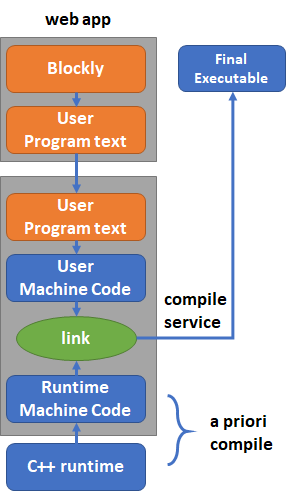
\includegraphics[width=1.5in]{images/bbc.png} & 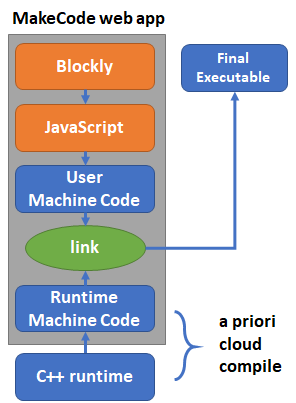
\includegraphics[width=1.5in]{images/makecode.png} \\
        (a) & (b) 
    \end{tabular}
    \caption{\label{fig:design}Web and compiler designs: (a) initial BBC design; (b) final design, as implemented in MakeCode.}
    \end{figure}

    
\subsection{The BBC micro:bit}

Main points:
\begin{itemize}
\item {\em A Visible Computer}: BBC micro:bit inherits the raw PCB nature of Arduino  (everything is visible to the end user).
\item {\em No Wiring}: makes starting easy
\item {\em Small Size}: 
\item {\em Scripting via Web App}: XYZ
\item {\em No Install}: XYZ
As shown in Figure~\ref{fig:design}(a), in the BBC design
the text of a user's program (whether derived from Blockly or produced directly by the user)
is submitted to a compile service that returns a final executable to be copied onto a micro:bit (connected to the host 
computer by USB) via a specialized loader application.  
avoiding the need for a compile service for user code (as shown 
in Figure~\ref{fig:design}(b));
\item {\em Extensible}: via edge connector and layered APIS (package system too).
\end{itemize}
From this perspective, the micro:bit can be seen as a starter device
for physical computing, embedded systems and cyber-physical systems, as it has
sensing, computation, control and networking capabilities built in.  The
micro:bit is not properly an IoT device, having no built-in way to connect
over IP, but it can be connected to other devices with IP connectivity. 

% Design considerations (technical requirements, steal from LCTES paper)

%   - hardware clearly distinguished from Arduino
%     - no wiring required to do interesting things (integrated sensors and outputs, etc.)
%     - device appears as USB pen drive (drag-and-drop programming)
 
%   - As with Arduino, embedding device into projects is essential (from beginner to maker)
%     - battery power
%     - works disconnected from host
%     - wearable, transportable
%     - low cost
%     - edge connector for easy connection to "shields"

%   - support for scripting languages (JavaScript and Python; no C/C++ for beginners)
%     - event-based programming model

%   - web-based IDE
%     - no apps or device drivers to install
%     - school considerations (minimize IT admin involvement)

%   - layered approach
%     - simple for absolute beginners to get started
%     - room for students to advance to more complex projects

% - worldwide rollout
%   - microbit.org, makecode.microbit.org

% from http://cacm.acm.org/system/assets/0000/6052/CACM_Author-Guidelines.pdf 

% 2.3.4 Contributed Articles
% Contributed Articles cover the wide and abundant spectrum of the computing field—its open challenges, 
% technical visions and perspectives, educational aspects, societal impact, significant applications and 
% research results of high significance and broad interest. 

% we have:
% + technical vision
% + educational aspect and societal impact
% + signification application
% - research results of high significance and broad interest: see LCTES 2018 article
